\chapter{Procesrapport}

\section{Læring og refleksion}
Der har været stort fokus på at udarbejde forskellige modeller og diagrammer gennem projektet. De er blevet brugt effektivt til at supplere både koordinering og planlægning af den kildekode som skulle udvikles. Der var en løbende justering af disse modeller, der blev lavet for at undgå problemer og fejl, som først blev opdaget efter first-cut udgaven var lavet. Hvis kildekoden var blevet produceret uden modeller og diagrammer, er det tydeligt at utallige fejl ville være opstået og hvis disse ikke blev løst ordentligt, kunne de have resulteret i et ubrugeligt system.\\
Brugen af brugsmønster modeller, analyse- og designdiagrammer mm. kan klart anbefales til fremtidige projekter, men med måde.\\
Der blev erfaret at tiden som blev brugt til at lave dynamiske diagrammer, ikke blev opvejet af værdien der kunne trækkes ud af dem. De blev brugt til at skabe fælles konsensus, om hvilken retning projektet skulle udvikles i, men var ikke præcise nok til at understøtte produktprogrammeringen.\\
Det er muligt at denne ulempe er et resultat af manglende erfaring med brugen af dynamiske diagrammer. At de blev introduceret sent i projektforløbet og var helt ny viden for gruppemedlemmerne, har sandsynligvis haft en stor indvirkning på hvor effektivt de blev brugt i projektet.\\
De statiske diagrammer er der kun blevet gjort positive erfaringer med. De blev brugt til at danne et klart grundlag for kildekoden, som gjorde at arbejdstempoet var højt og er løbende blevet brugt til at sikre at klasser blev skrevet korrekt. Den succes som der er blevet gjort med de statiske diagrammer, har gjort det tydeligt, hvor nyttig og essentielt planlægning er for et succesfuldt projekt.  
\newpage
\section{Projektstyring}
Projektplanlægning bruges til at udarbejde estimater for hvor lang tid en given opgave vil tage at fuldende og derved også give en estimeret tidsplan for et projekt.\\
Projektstyring bruges til at bestemme hvordan en opgave kan udføres mest effektivt, hvor mange ressourcer der skal bruges på den og for at sikre de estimater der er blevet stillet i planlægningen ikke overskrides med for stor en margin, hvis den overhovedet overskrides.\\
Til projektets planlægning blev der udarbejdet en række milepæle, samt der blev lagt en tidsplan for hvornår de forskellige milepæle skulle være nået. Milepælene blev oprettet i github så vi havde dem placeret et centralt sted som alle havde adgang til. 
\begin{figure}[h]
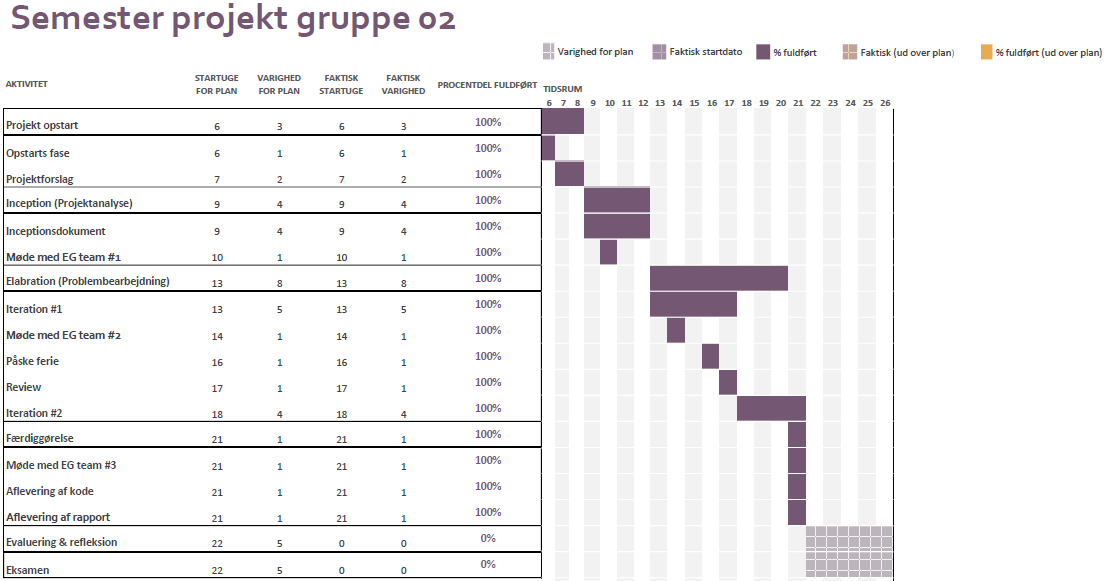
\includegraphics[width = \linewidth]{./PNG/proces/tidsplan.png}
\caption{Tidsplan se interne bilag \ref{sec:diverse} figur \ref{fig:tidsplanf}}
\label{fig:tidsplan}
\end{figure}
Til styring af projektet er der blevet brugt værktøjet GitKraken Glo, til at håndtere projektets kanban board, som bestod af issues oprettet i githubs issue-tracking system. For at sikre et godt overblik kunne issues være i forskellige stadier ”Issues”, ”To Do”, ”In Progress” og ”Need review”. På denne måde var det muligt at se hvor langt en given opgave var nået. \\
Hvis en opgave var i stadiet ”Issues”, betød det at den manglede at blive tildelt til en i gruppen. \\
Hvis en opgave var i stadiet ”To Do”, betød det at den var blevet tildelt en person, men ikke var startet.\\
Hvis en opgave var i stadiet ”In Progress”, betød det at den var ved at blive løst.\\
Hvis en opgave var i stadiet ”Need review”, betød det at den var løst og skulle gennemgås af gruppen.\\
\begin{figure}[h]
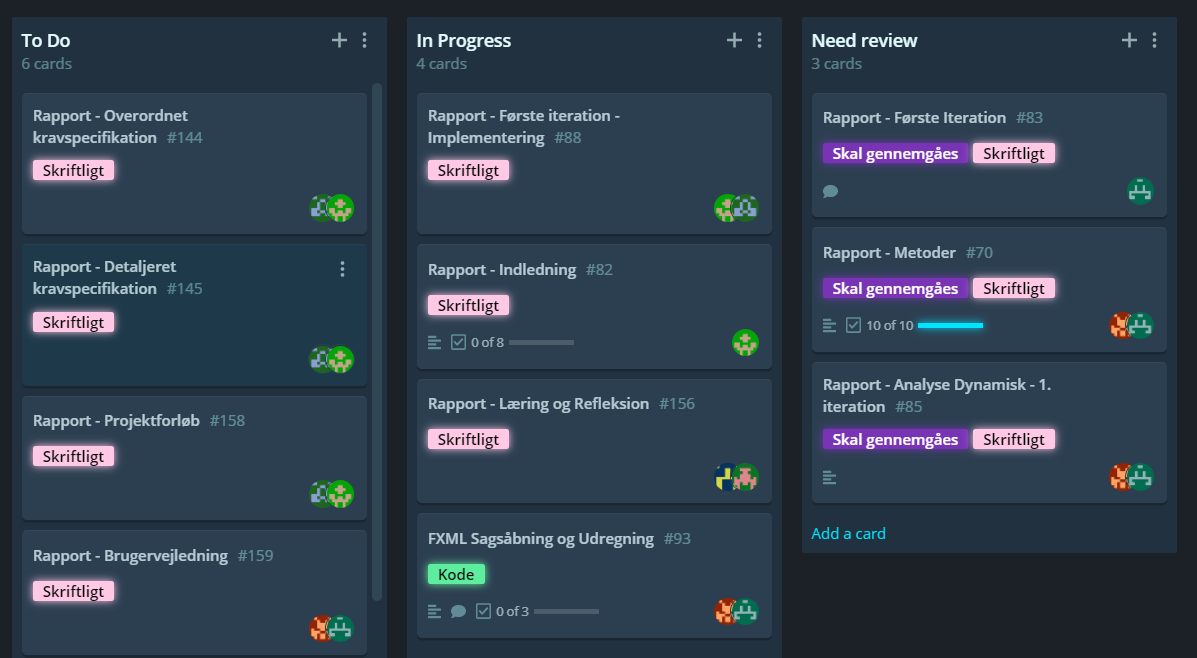
\includegraphics[width = \linewidth]{./PNG/proces/kanban.png}
\caption{Kanban board se interne bilag \ref{sec:diverse} figur \ref{fig:tidsplanf}}
\label{fig:kanban}
\end{figure}
Der blev holdt to ugentlige møder, tirsdag og fredag, for at fordele eksisterende opgaver og for at oprette nye, som opstod i forlængelse af udviklingen. Tirsdagsmødet inkluderede et vejledermøde, som blev brugt til at få feedback på det udførte arbejde og planerne gruppen havde lagt for fremtidigt arbejde. Vejledermødet blev også brugt til at forventningsafstemme, hvordan nyt materiale skulle bruges og vægtes, hvis der var tvivl om dette.\\
\textbf{Ansvarsfordeling}
\begin{itemize}
\item Planlægger: gitkraken, issue: Aleksander H. 
\item Ordstyrer, dagsorden i forhold til møder: Aslak 
\item Referent: Steffen og Aleksander D. 
\item Rapporten: Per og Mathias. 
\end{itemize}
\newpage
\section{Identifikation, analyse og bearbejdning af problemer}
\subsection{Misforståelser}
Det største problem som der har været gennem projektarbejdet, har været misforståelser. Disse misforståelser er primært opstået på grund af forkert brug af fagtermer og dårlig formulering, og kan generelt beskrives som dårlig kommunikation.\\
Når der har været en diskussion mellem to parter og det ikke har været muligt at komme til enighed, afbrydes diskussionen og én af parterne får så ordet. Første part får så chancen for at uddybe deres holdninger, og anden part stiller uddybende spørgsmål til disse. Hvis parterne ikke er kommet til enighed, bliver rollerne byttet, anden part uddyber og første part stiller spørgsmål.\\
Ved at arbejde med én holdning ad gangen, er det muligt at få en klar forståelse for det perspektiv som der argumenteres ud fra og på denne måde identificeres den eventuelle misforståelse og et kompromis kan indgås hvis nødvendigt.
\subsection{Faglighed}
Den løbende introduktion af nye emner, har givet problemer gennem projektet. Efter at der er blevet introduceret ny teori, har der til tider været problemer med forståelsen af dette, på grund af fejllæsninger eller mistolkning af teori. Nogle gange har der ikke været en fælles forståelse for et givent emne, som har afsporet arbejdet.\\
Når dette er skete, blev teorien gennemgået i plenum, for at ensrette forståelsen. Når alle teoriens aspekter var gennemgået, blev arbejdet genoptaget og typisk ville problemet så være løst.
\section{Udviklingsprocessen}
De faser som udviklingsprocessen ligger vægt i er Inceptions- og Elaborationsfasen, hvor Elaborationsfasen har været opdelt i to iterationer, disse iterationer er skulle deles op efter brugsmønstre, gruppen valgt at ligge vægt på både opret sag og find sag i begge iterationer, første iteration gik dog ud på at lave et domæne lag som der kunne arbejdes videre ud fra i anden iteration.\\
I Inceptionsfasen har gruppen haft fokus på at udarbejde aktørliste, brugsmønstre med kortebeskrivelse, samt en beskrivelse af hvad der skal gennemgås for at udføre de givende brugsmønstre. Denne detaljering af brugsmønstre beskrivelsen havde først været forventet at blive udført i løbet af Elaborationsfasen efterhånden som man begynder at arbejde med de enkelte brugsmønstre. Der er dertil også blevet udarbejdet et overordnet brugsmønsterdiagram med systemafgrænsning, som viser hvilken aktører deres kan interagere med hvilken brugsmønstre i systemet. Der blev også i Inceptionsfasen lavet et first-cut domæne klasse diagram, hvilket skulle have været udarbejdet i løbet af Elaborationsfasen efterhånden som der blevet arbejdet med de forskellige brugsmønstre.\\
I Elaborationsfasen har gruppen arbejdet ud fra brugsmønstrene opret sag og søg sag, her er det blevet udarbejdet sekvinsdiagrammer til at forklar hvordan systemet gennemløber brugsmønstre, sekvinsdiagrammer har fået tilføjet metode navne med parameter. Der er blevet udarbejdet kontrakter, som giver en forklaring af hvad de forskellige metoder indenfor brugsmønstrene skal stå for og hvad man kan forvente at få af output fra dem, samt hvad der skal gøres før metoden virker. Der er i designfasen af Elaborationsfasen blevet udarbejdet et arkitektonisk sekvinsdiagram, som fortæller hvad der sker når bruger arbejder med systemet. Der blev også i designfasen udarbejdet et analyse klasse diagram som blev udarbejdet så metoder og klasser stod klar til implementering, i implementeringsfasen blev der lagt vægt på at få et grafisk udseende for opret sag og søg sag, samt få lavet logikken i domænet og persistens laget, så det giver et indblik i hvad gruppen havde tænkt sig hvis projektet gik videre til den næste fase af Unified Proces.

\section{Formidling og kommunikation}
Gruppen har haft 1-2 ugentlige møder hvor vi har siddet på Syddansk Universitet og snakke om hvad de forskellige parproduktionsgrupper har nået siden vi sidst snakket sammen. Hvis der er nogen af grupperne som ikke har nået det vi havde aftale sad vi sammen som en fælles gruppe og lavet de forskellige ting, inden dagens møde sluttet aftale gruppen hvad der skulle ske til næste gang og aftale en dagsorden for næste dag, og hvis det næste møde lå til en tirsdag blev der også lavet en dagsorden til vejledermødet og sendt til vejleder hvis der var noget punkter til dette møde. Til at kommunikere har gruppen benyttet undervisnings dage, såvel som Facebook og Discord. Facebook er blevet brugt til lette beskeder, så som hvis nogen er syge eller forsinket til et møde. Discord er blevet brugt til beskeder af lidt mere substans, hvor der intet er krævet et telefonisk møde eller video chat, for at hvis hvad man mangler hjælp til eller et evt. svar til det stillede spørgsmål. Discord er også blevet brugt til at holde nogen af de ugentlige møder i tilfælde af at der har enighed om at parproduktionsgrupperne har kunne arbejde hjemme fra, så er der blevet holdt et opsumeringsmøde midt eller sidst på dagen så alle i projektgruppen er uptodate med hvad der er sket.
\section{Samarbejde i gruppen}
Gruppen har arbejdet med parproduktion, hvor grupperne har ændret sig fra iteration til iteration eller når noget andet større begyndte. Dette har været en fordel for gruppen at der var en marker at spørge før et spørgsmål noget ud til gruppen. Dette har været med til at gøre at de spørgsmål der blev stillet i gruppen var mere præcise, da de allerede var kommet et input fra en anden person, som ofte har kunnet svare på dele hvis ikke hele spørgsmålet. \\
Genneralt set har gruppen fungeret godt, med at der ikke var større problemer. Dette mener vi selv skyldes at gruppedynamikken blev sat fast tidligt, men ikke så fast at der ikke var til at udvikle sig igennem projektet. Der har været nogle misforståelser under vejs, som er håndteret som skrevet tidligere hvilket har været med til at skabe en større forståelse i gruppen. 
\section{Samarbejde med vejleder}
Gruppen har haft et godt samarbejde med Henrik, når gruppen har haft nogen spørgsmål omhandlende dele af projektet er han kommet med et svar som inden har givet gruppen en dybere forståelse for problemet ellers har han formået at give en feedback så det har været muligt at se opgaven fra et andet synspunkt og derved også gøre det muligt at løseproblemet uden yderlige hjælp. Henrik har altid mødt velforberedt op til vejleder møderne og vist at han ønsker at gruppen har lykkes med de opgaver som har været et problem for gruppen, hertil har Henrik også altid været forberedt på at gruppen kommer med et problem som ikke er blevet oplyst til ham på forhånd, men stadig indenfor meget kort til kunne komme med en løsning, om det så har været til udarbejdning af diagrammer eller selve implementering.





\newpage